% Standard Paper
\documentclass[letterpaper, 10 pt, conference]{ieeeconf}

% A4 Paper
%\documentclass[a4paper, 10pt, conference]{ieeeconf}      

% Only needed for \thanks command
\IEEEoverridecommandlockouts

% Needed to meet printer requirements.
\overrideIEEEmargins

%In case you encounter the following error:
%Error 1010 The PDF file may be corrupt (unable to open PDF file) OR
%Error 1000 An error occurred while parsing a contents stream. Unable to analyze the PDF file.
%This is a known problem with pdfLaTeX conversion filter. The file cannot be opened with acrobat reader
%Please use one of the alternatives below to circumvent this error by uncommenting one or the other
%\pdfobjcompresslevel=0
%\pdfminorversion=4

% See the \addtolength command later in the file to balance the column lengths
% on the last page of the document

% The following packages can be found on http:\\www.ctan.org
\usepackage{graphicx} % for pdf, bitmapped graphics files
%\usepackage{epsfig} % for postscript graphics files
%\usepackage{mathptmx} % assumes new font selection scheme installed
%\usepackage{times} % assumes new font selection scheme installed
%\usepackage{amsmath} % assumes amsmath package installed
%\usepackage{amssymb}  % assumes amsmath package installed
\usepackage{url}

\hyphenation{analysis}

\title{\LARGE \bf HRIStudio: A Framework for Wizard-of-Oz Experiments in Human-Robot Interaction Studies}

\author{Sean O'Connor and L. Felipe Perrone$^{*}$
    \thanks{$^{*}$Both authors are with the Department of Computer Science at
        Bucknell University in Lewisburg, PA, USA. They can be reached at {\tt\small sso005@bucknell.edu} and {\tt\small perrone@bucknell.edu}}%
}

\begin{document}

\maketitle
\thispagestyle{empty}
\pagestyle{empty}


%%%%%%%%%%%%%%%%%%%%%%%%%%%%%%%%%%%%%%%%%%%%%%%%%%%%%%%%%%%%%%%%%%%%%%%%%%%%%%%%
\begin{abstract}

Human-robot interaction (HRI) research plays a pivotal role in shaping how robots communicate and collaborate with humans. However, conducting HRI studies, particularly those employing the Wizard-of-Oz (WoZ) technique, presents challenges due to technical complexities and specialized expertise requirements. To address these challenges, we propose HRIStudio, a novel web-based platform designed to streamline the design, execution, and analysis of WoZ experiments in HRI research. HRIStudio offers an intuitive interface for experiment creation, real-time control and monitoring during live sessions, and comprehensive data logging and playback tools for analysis and reproducibility. By lowering technical barriers and promoting collaboration, HRIStudio aims to accelerate innovation in human-centered robotics research, empowering researchers to explore novel HRI concepts efficiently and effectively.

\end{abstract}


%%%%%%%%%%%%%%%%%%%%%%%%%%%%%%%%%%%%%%%%%%%%%%%%%%%%%%%%%%%%%%%%%%%%%%%%%%%%%%%%

%% TODO: Update mockup pictures with photo of subject and robot

\section{Introduction}

Human-robot interaction (HRI) is an essential field of study for understanding how robots should communicate, collaborate, and coexist with people. The development of autonomous behaviors in social robot applications, however, offers a number of challenges. The Wizard-of-Oz (WoZ) technique has emerged as a valuable experimental paradigm to address these difficulties, as it allows experimenters to simulate a robot's autonomous behaviors. With WoZ, a human operator (the \emph{``wizard''}) can operate the robot remotely, essentially simulating its autonomous behavior during user studies. This enables the rapid prototyping and continuous refinement of human-robot interactions postponing to later the full development of complex robot behaviors.

While WoZ is a powerful paradigm, it does not eliminate all experimental challenges. Researchers may face barriers related to the use of specialized tools and methodologies involved in WoZ user studies and also find difficulties in creating fully reproducible experiments. Existing solutions often rely on low-level robot operating systems, limited proprietary platforms, or require extensive custom coding, which can restrict their use to domain experts with extensive technical backgrounds.

Through a comprehensive review of current literature, we have identified a pressing need for a platform that simplifies the process of designing, executing, analyzing, and recording WoZ-based user studies. To address this gap, we are developing \emph{HRIStudio},  a novel web-based platform that enables the intuitive configuration and operation of WoZ studies for HRI research. Our contribution leverages the \emph{Robot Operating System} (ROS) to handle the complexities of interfacing with different robotics platforms. HRIStudio presents users with a high-level, user-friendly interface for experimental design, live control and monitoring, and comprehensive post-study analysis. The system offers drag-and-drop visual programming for describing experiments without extensive coding, real-time control and observation capabilities during live experiment sessions, as well as comprehensive data logging and playback tools for analysis and enhanced reproducibility. We expect that with these features, HRIStudio will increase the usability of the  WoZ paradigm and increase scientific rigor of HRI experiments. The following sections outline our proposed system design, experimental workflow structure, implementation progress, and future directions for this work.

\section{State-of-the-Art}

The importance of the WoZ paradigm for user studies in social robotics is illustrated by the several frameworks that have been developed to support it. We describe some of the most notable as follows.

\emph{Polonius}~\cite{Lu2011}, which is based on the modular ROS platform, offers a graphical user interface for wizards to define finite state machine scripts that drive the behavior of robots during experiments. \emph{NottReal}~\cite{Porcheron2020} was designed for WoZ studies of voice user interfaces. It provides scripting capabilities and visual feedback to simulate autonomous behavior for participants. \emph{WoZ4U}~\cite{Rietz2021} presents a user-friendly GUI that makes HRI studies more accessible to non-programmers. The tight hardware focus on Aldebaran's Pepper, however, constrains the tool's applicability. \emph{OpenWoZ}~\cite{Hoffman2016} proposes a runtime-configurable framework with a multi-client architecture, enabling evaluators to modify robot behaviors during experiments. The platform allows one with programming expertise to create standard, customized robot behaviors for user studies.

In addition to the aforementioned frameworks, we considered Riek's systematic analysis of published WoZ experiments, which stresses the need for increased methodological rigor, transparency and reproducibility of WoZ studies.~\cite{Riek2012} Altogether, the literature inspired us to design HRIStudio as a platform that offers comprehensive support for WoZ studies in social robotics. Our design goals include offering a platform that is as ``robot-agnostic'' as possible and which offers its users guidance to specify and execute WoZ studies that are methodologically sound and maximally reproducible. As such, HRIStudio aims to offer an easy user interface that allows for experiments to be scripted and executed easily and which allows for the aggregation of experimental data and other assets generated in a study.

\section{Overarching Design Goals}

We have identified several guiding design principles to maximize HRIStudio's effectiveness, usefulness, and usability. Foremost, we want HRIStudio to be accessible to users with and without deep robot programming expertise so that we may lower the barrier to entry for those staging HRI studies. The platform should provide an intuitive graphical user interface that obviates the need for describing robot behaviors in a programming language. The user should be able to focus on describing sequences of robot behaviors without getting bogged down by all the details of specific robots. To this end, we determined that the framework should offer users the means by which to describe experiments and robot behaviors, while capturing and storing all data generated including text-based logs, audio, video, IRB materials, and user consent forms. 

Furthermore, we determined that the framework should also support multiple user accounts and data sharing to enable collaborations between the members of a team and the dissemination of experiments across different teams. By incorporating these design goals, HRIStudio prioritizes experiment design, collaborative workflows, methodological rigor, and scientific reproducibility.

\section{Design of the Experimental Workflow}

\subsection{Organization of a user study}

With HRIStudio, we define a hierarchical organization of elements to express WoZ user studies for HRI research. An experimenter starts by creating and configuring a \emph{study} element, which will comprise multiple instantiations of one same experimental script encapsulated in an element called \emph{experiment}, which captures the experiences of a specific human subject with the robot designated in the script. 

Each \emph{experiment} comprises a sequence of one or more \emph{step} elements. Each \emph{step} models a phase of the experiment and aggregates a sequence of \emph{action} elements, which are fine-grained, specific tasks to be executed either by the wizard or by the robot. An \emph{action} targeted to the wizard provides guidance and maximizes the chances of consistent behavior. An \emph{action} targeted at the robot causes it to execute movements or verbal interactions, or causes it to wait for a human subject's input or response.

The system executes the \emph{actions} in an experimental script asynchronously and in an event-driven manner, guiding the wizard's behavior and allowing them to simulate the robot's autonomous intelligence by responding to the human subject in real time based on the human's actions and reactions. This event-driven approach allows for flexible and spontaneous reactions by the wizard, enabling a more natural and intelligent interaction with the human subject. In contrast, a time-driven script with rigid, imposed timing would show a lack of intelligence and autonomy on the part of the robot.

In order to enforce consistency across multiple runs of the \emph{experiment}, HRIStudio uses specifications encoded in the \emph{study} element to inform the wizard on how to constrain their behavior to a set of possible types of interventions. Although every experiment is potentially unique due to the unlikely perfect match of reactions between human subjects, this mechanism allows for annotating the data feed and capturing the nuances of each unique interaction.

Figure~\ref{fig:userstudy} illustrates this hierarchy of elements with a practical example.  We argue that this hierarchical structure for the experimental procedure in a user study benefits methodological rigor and reproducibility while affording the researcher the ability to design complex HRI studies while guiding the wizard to follow a consistent set of instructions.

\begin{figure}[ht]
   \vskip -0.3cm
    \begin{center}
        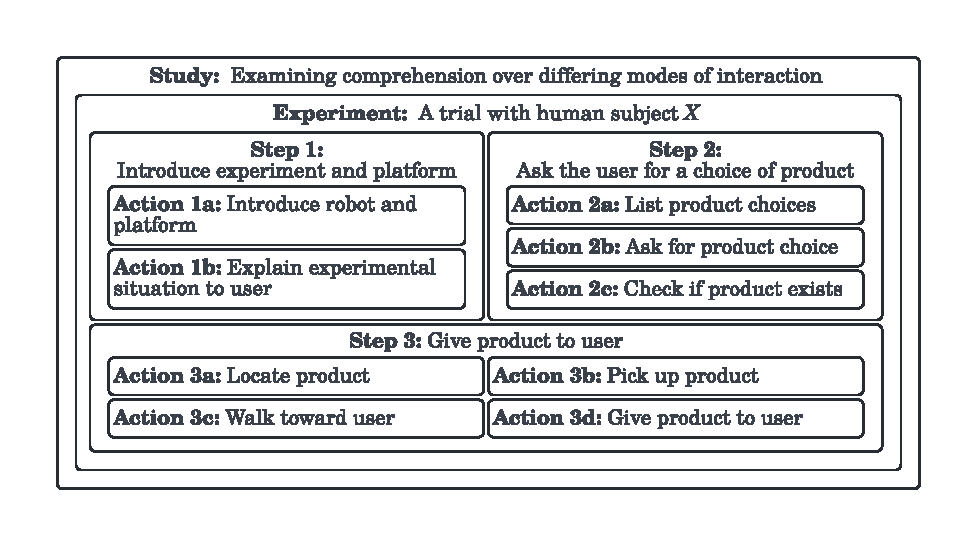
\includegraphics[width=0.4\paperwidth]{assets/diagrams/userstudy}
        \vskip -0.5cm
        \caption{A sample user study.}
        \label{fig:userstudy}
    \end{center}
\vskip -0.7cm
\end{figure}

\subsection{System interfaces} 

HRIStudio features a user-friendly graphical interface for designing WoZ experiments. This interface provides a visual programming system that allows one to build their experiments using a drag-and-drop approach. The core of the experiment creation process offers a library of actions including common tasks and behaviors executed in the experiment such as robot movements, speech synthesis, and instructions for the wizard. One can drag and drop action components onto a canvas and arrange them into sequences that define  study, experiment, steps, and action components. The interface provides configuration options that allow researchers to customize parameters in each element. This configuration system offers contextual help and documentation to guide researchers through the process while providing examples or best practices for designing studies.

\subsection{Live experiment operation}

During live experiment sessions, HRIStudio offers multiple synchronized views for experiment execution and observation, and data collection. The wizard's \emph{Execute} view gives the wizard control over the robot's actions and behaviors. Displaying the current step of the experiment along with associated actions, this interface facilitates intuitive navigation through the structural elements of the experiments and allows for the creation of annotations on a timeline. The wizard can advance through actions sequentially or manually trigger specific actions based on contextual cues or responses from the human subject. During the execution of an experiment, the interface gives the wizard manual controls to insert unscripted robot movements, speech synthesis, and other functions dynamically. These events are recorded in persistent media within the sequence of actions in the experimental script.

In parallel, the observer's \emph{Execute} view supports live monitoring, note-taking, and potential interventions by additional researchers involved in the experiment. This feature ensures the option of continuous oversight without disrupting the experience of human subjects or the wizard's control. Collaboration on an experiment is made possible by allowing multiple observers to concurrently access the \emph{Execute} view.

\subsection{Data logging, playback, and annotation}

Throughout the live experiment session, the platform automatically logs various data streams, including timestamped records of all executed actions and experimental events, exposed robot sensor data, and audio and video recordings of the participant's interactions with the robot. This logged data is stored in JavaScript Object Notation (JSON)  encrypted files kept in secure storage, enabling efficient post-experiment data analysis without compromise to the privacy of human subjects.

After a live experiment session, researchers may use a \emph{Playback} view to inspect the recorded data streams and develop a holistic understanding of the experiment's progression. This interface supports features such as playback of recorded data such as audio, video, and sensor data streams, scrubbing of recorded data with the ability to mark and note significant events or observations, and export options for selected data segments or annotations.

\section{Implementation}

The realization of the proposed platform is a work in progress. So far, we have made significant advances on the design of the overall framework and of its several components while exploring underlying technologies, wireframing user views and interfaces, and establishing a development roadmap.

\subsection{Core technologies used}

We are leveraging the \emph{Next.js React} \cite{next} framework for building our framework as a web application. Next.js provides server-side rendering, improved performance, and enhanced security. By making HRIStudio a web application, we achieve independence from hardware and operating system. We are building into the framework support for API routes and integration with \emph{TypeScript Remote Procedure Call} (tRPC), which simplifies the development of APIs for interfacing with the ROS interface.

For the robot control layer, we utilize ROS as the communication and control interface. ROS offers a modular and extensible architecture, enabling seamless integration with a multitude of consumer and research robotics platforms. Thanks to the widespread adoption of ROS in the robotics community, HRIStudio will be able to support a wide range robots out-of-the-box by leveraging the  efforts of the ROS community for new robot platforms.

\subsection{High-level architecture}

We have designed our system as a full-stack web application.  The frontend handles user interface components such as the experiment \emph{Design} view, the experiment \emph{Execute} view, and the \emph{Playback} view. The backend API logic manages experiment data, user authentication, and communication with a ROS interface component. In its turn, the ROS interface is implemented as a separate C++ node and translates high-level actions from the web application into low-level robot commands, sensor data, and protocols, abstracting the complexities of different robotics platforms. This modular architecture leverages the benefits of Next.js' server-side rendering, improved performance, and security, while enabling integration with various robotic platforms through ROS.

\begin{figure}[ht]
   \vskip -0.3cm
    \begin{center}
        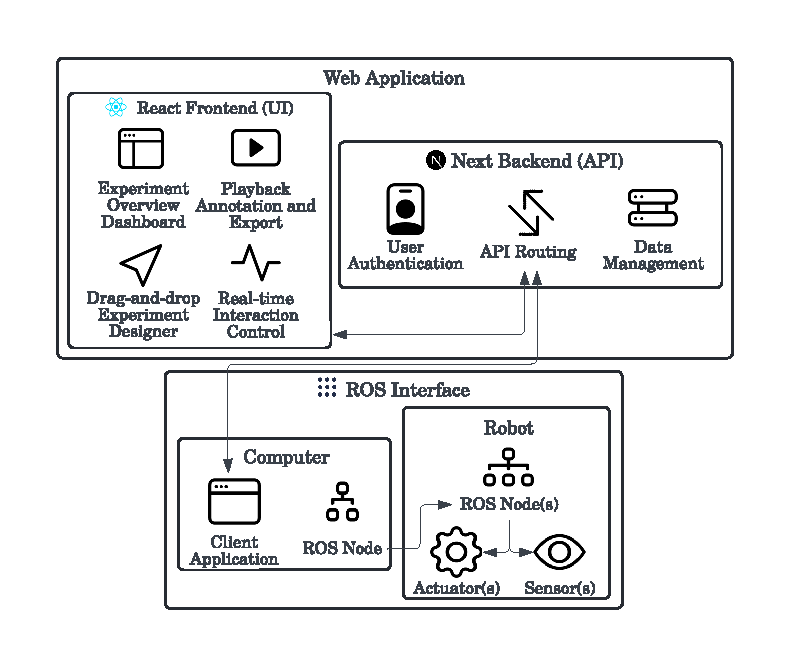
\includegraphics[width=0.4\paperwidth]{assets/diagrams/systemarch}
        \vskip -0.3cm
        \caption{The high-level system architecture of HRIStudio}
        \label{fig:systemarch}
    \end{center}
     \vskip -0.7cm
\end{figure}

\subsection{User interface mockups}

A significant portion of our efforts have been dedicated to designing intuitive and user-friendly interface mockups for the platform's key components. We have created wireframes and prototypes for the study \emph{Dashboard}, \emph{Design} view, \emph{Execute} view, and the \emph{Playback} view.

The study \emph{Dashboard} mockups (see Figure~\ref{fig:dashboard}) display an intuitive overview of a project's status, including platform information, collaborators, completed and upcoming trials, subjects, and a list of pending issues. This will allow a researcher to quickly see what needs to be done, or easily navigate to a previous trial's data for analysis.

\begin{figure}[h]
    \begin{center}
        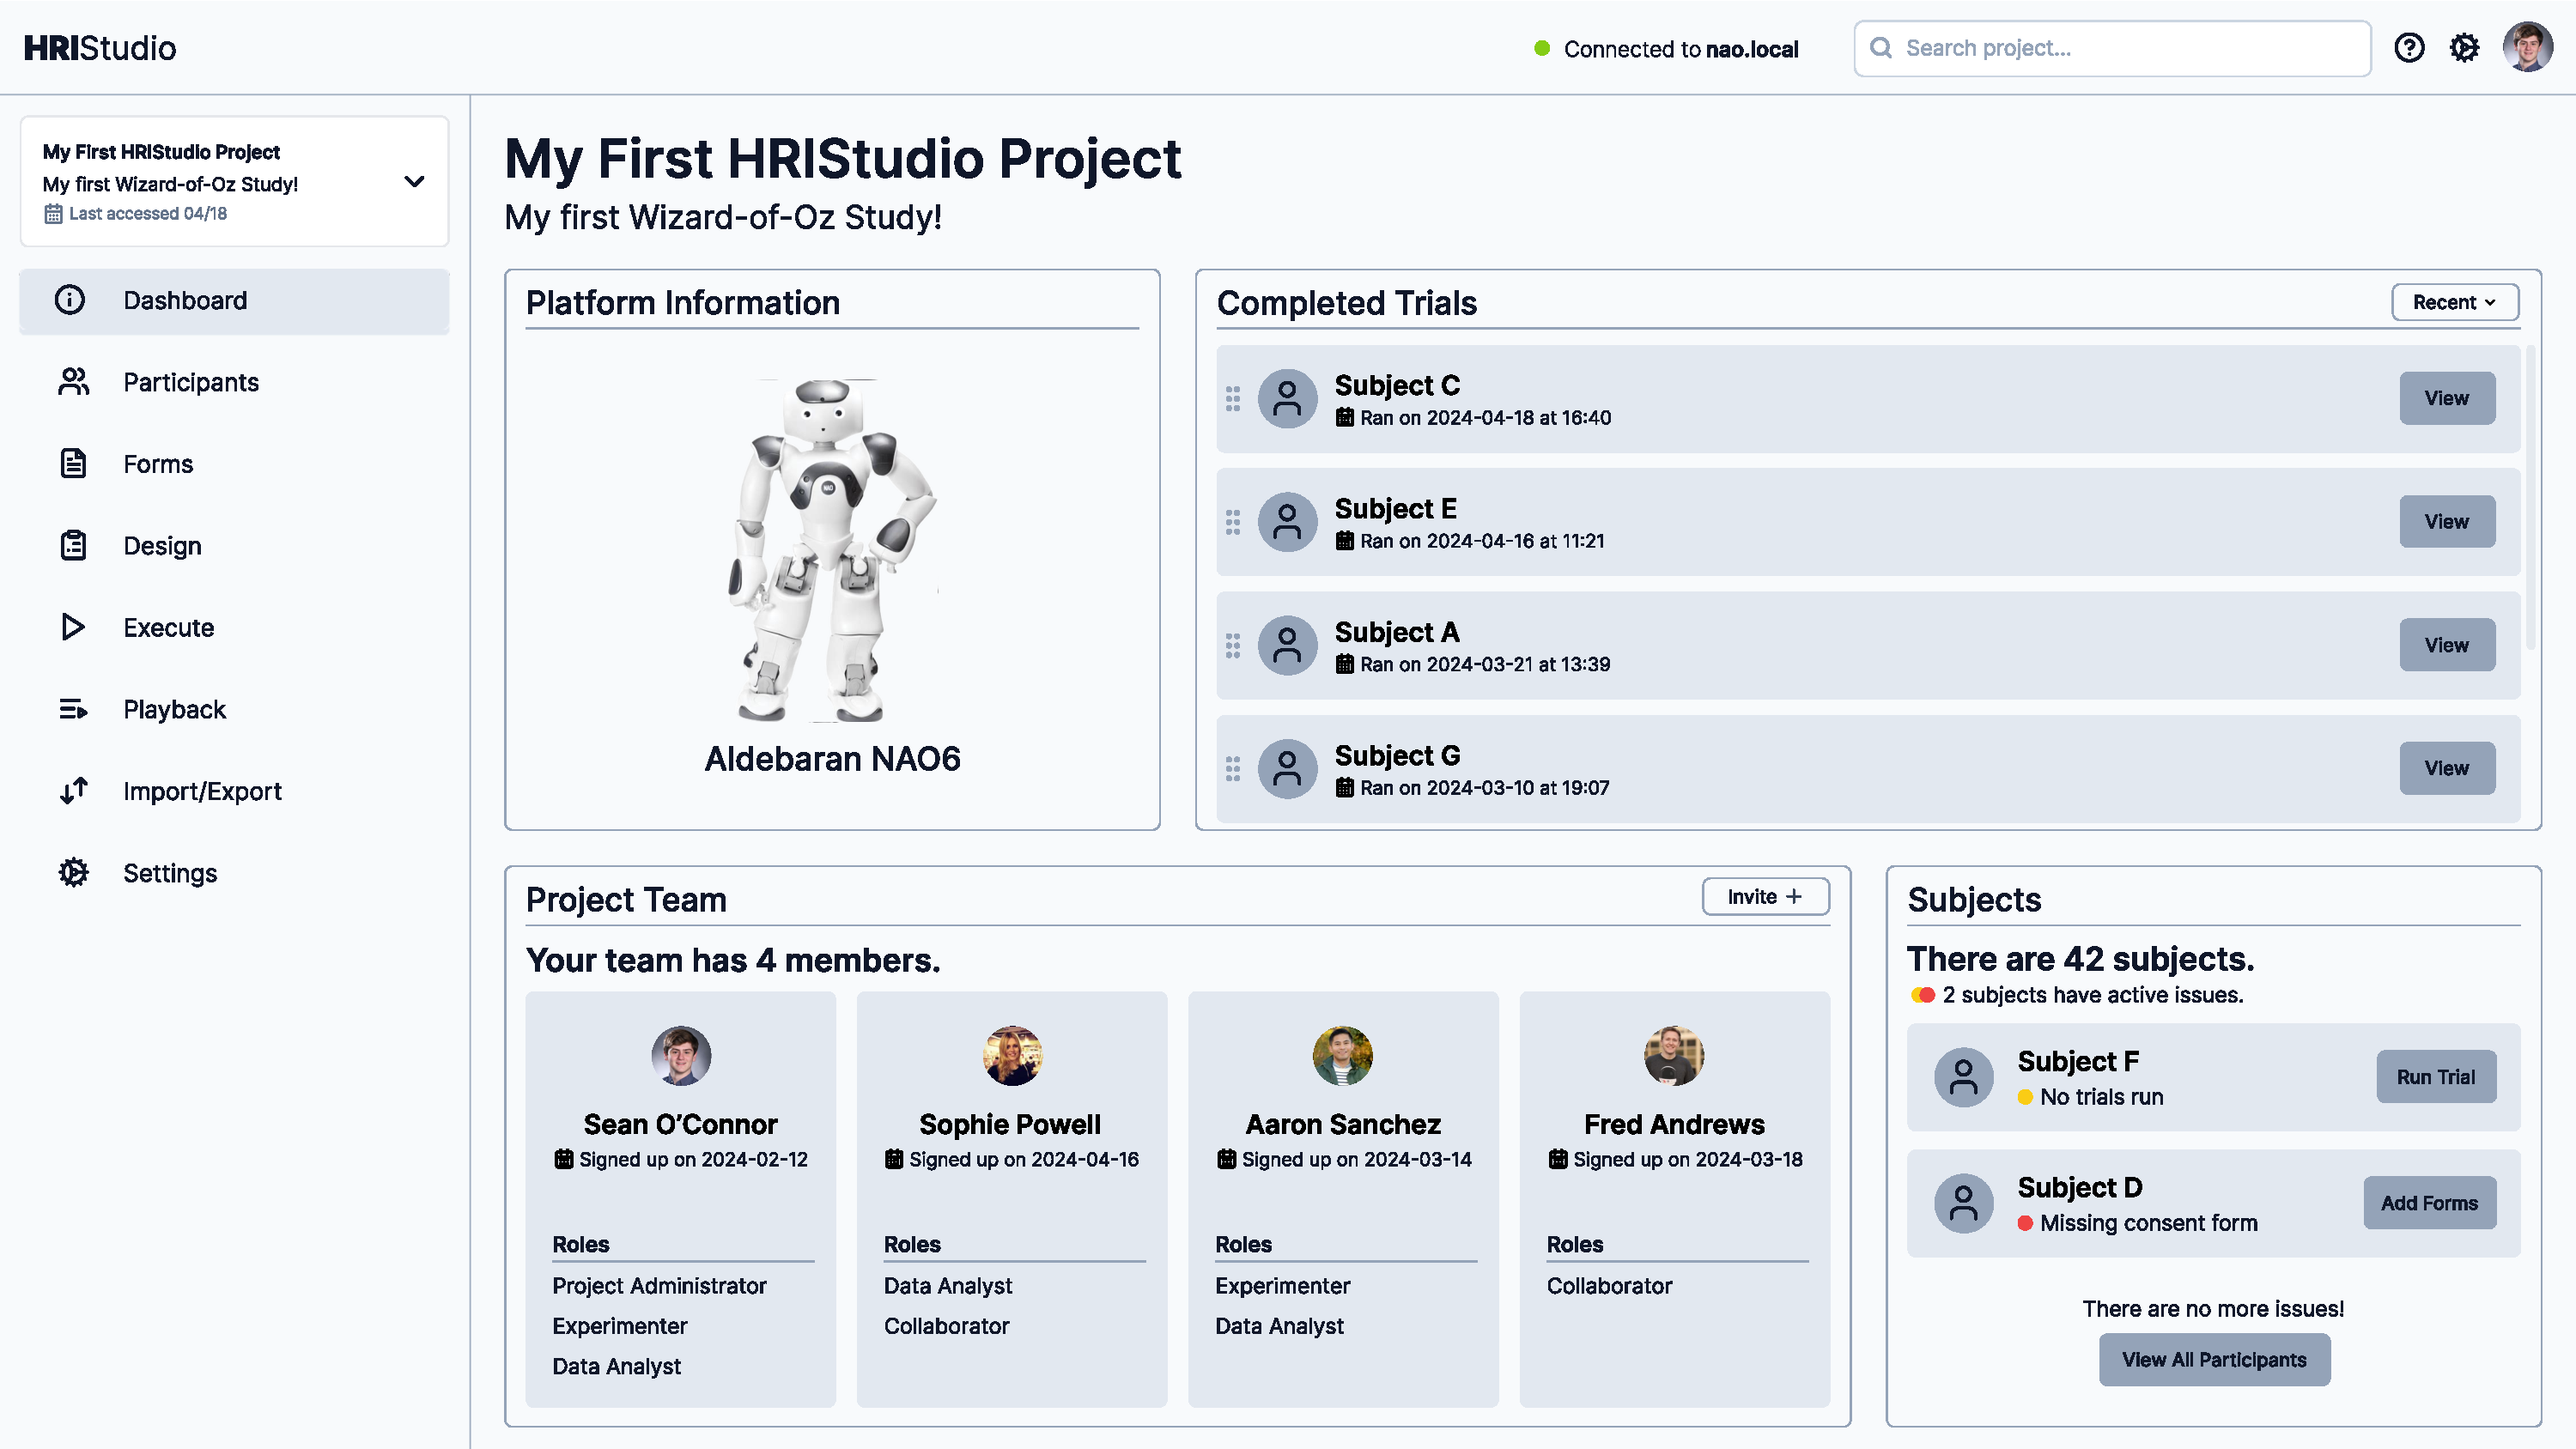
\includegraphics[width=0.4\paperwidth]{assets/mockups/dashboard}
        \vskip -0.3cm
        \caption{A sample project's \emph{Dashboard} view within HRIStudio}
        \label{fig:dashboard}
    \end{center}
    \vskip -0.4cm
\end{figure}

The \emph{Design} view mockups depicted in Figure~\ref{fig:design} feature a visual programming canvas where researchers can construct their experiments by dragging and dropping pre-defined action components. These components represent common tasks and behaviors, such as robot movements, speech synthesis, and instructions for the wizard. The mockups also include configuration panels for customizing the parameters of each action component.

\begin{figure}[h]
    \begin{center}
        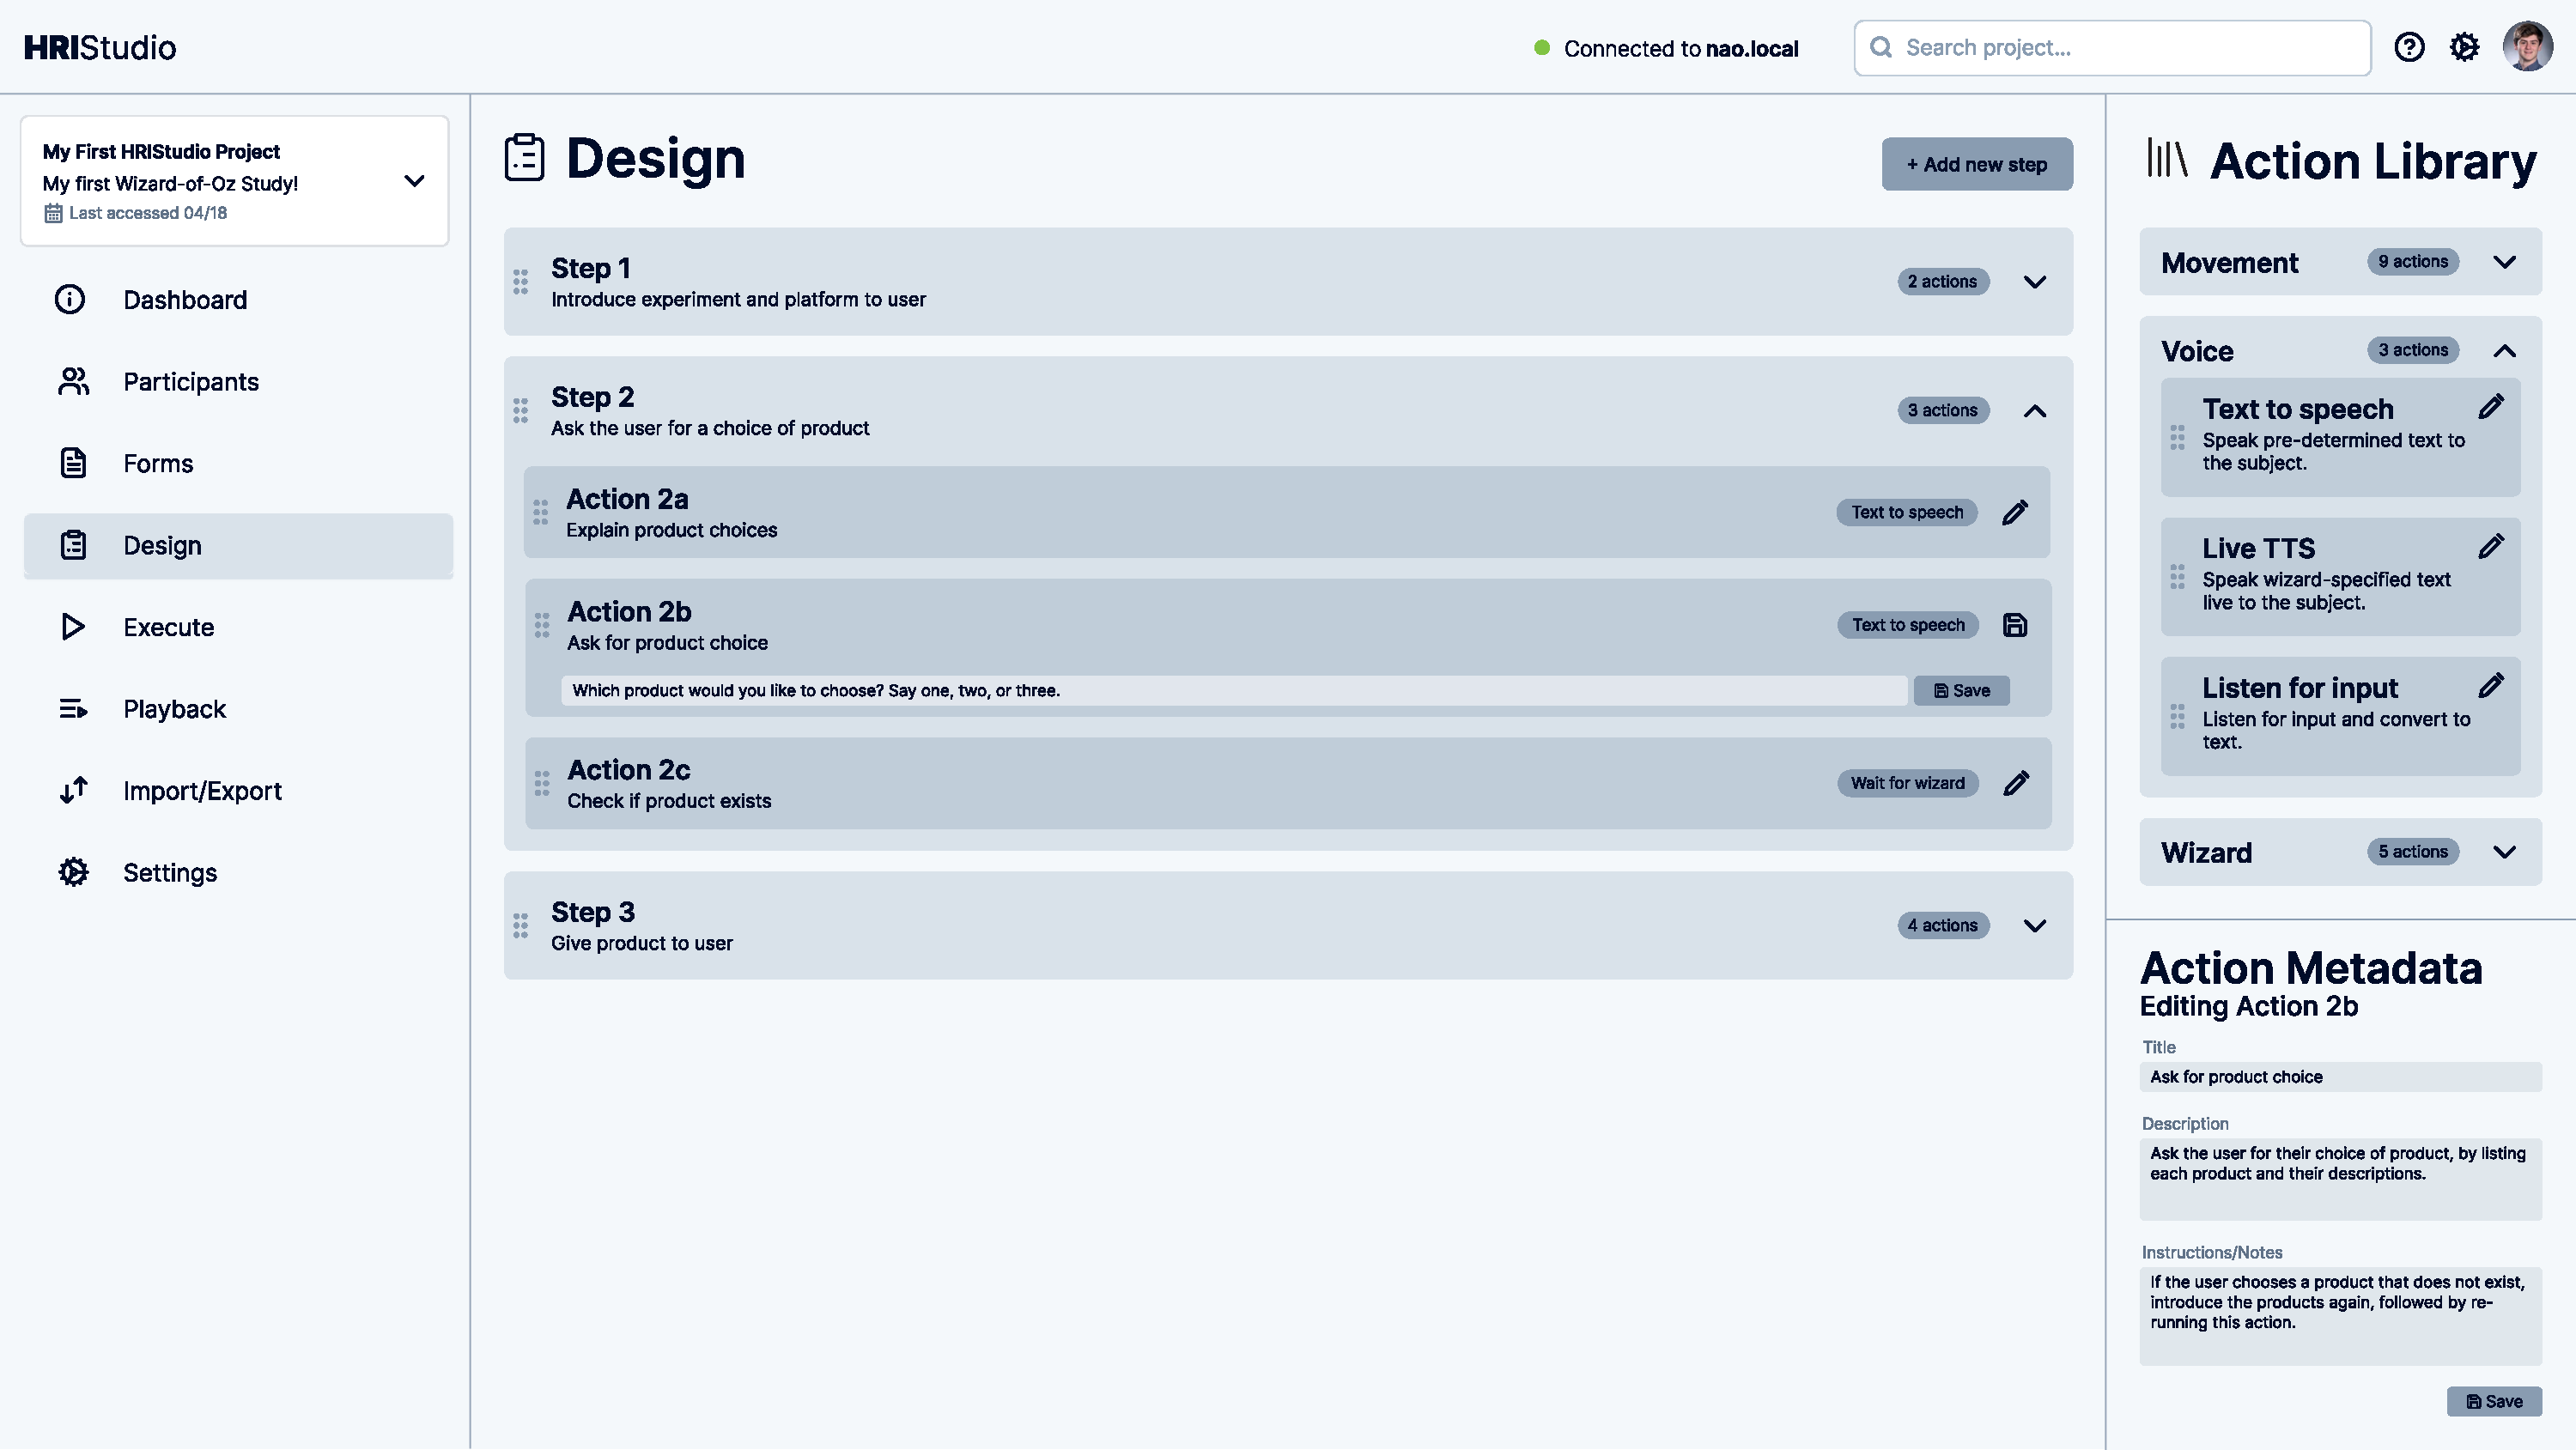
\includegraphics[width=0.4\paperwidth]{assets/mockups/design}
         \vskip -0.3cm
        \caption{A sample project's \emph{Design} view in HRIStudio}
        \label{fig:design}
    \end{center}
    \vskip -0.5cm
\end{figure}

For the \emph{Execute} view, we have designed mockups that provide synchronized views for the wizard and observers. The wizard's view (see Figure~\ref{fig:execute}) presents an intuitive step-based interface that walks the wizard through the experiment as specified by the designer, triggering actions, and controlling the robot, while the observer view facilitates real-time monitoring and note taking.

\begin{figure}[h]
    \begin{center}
        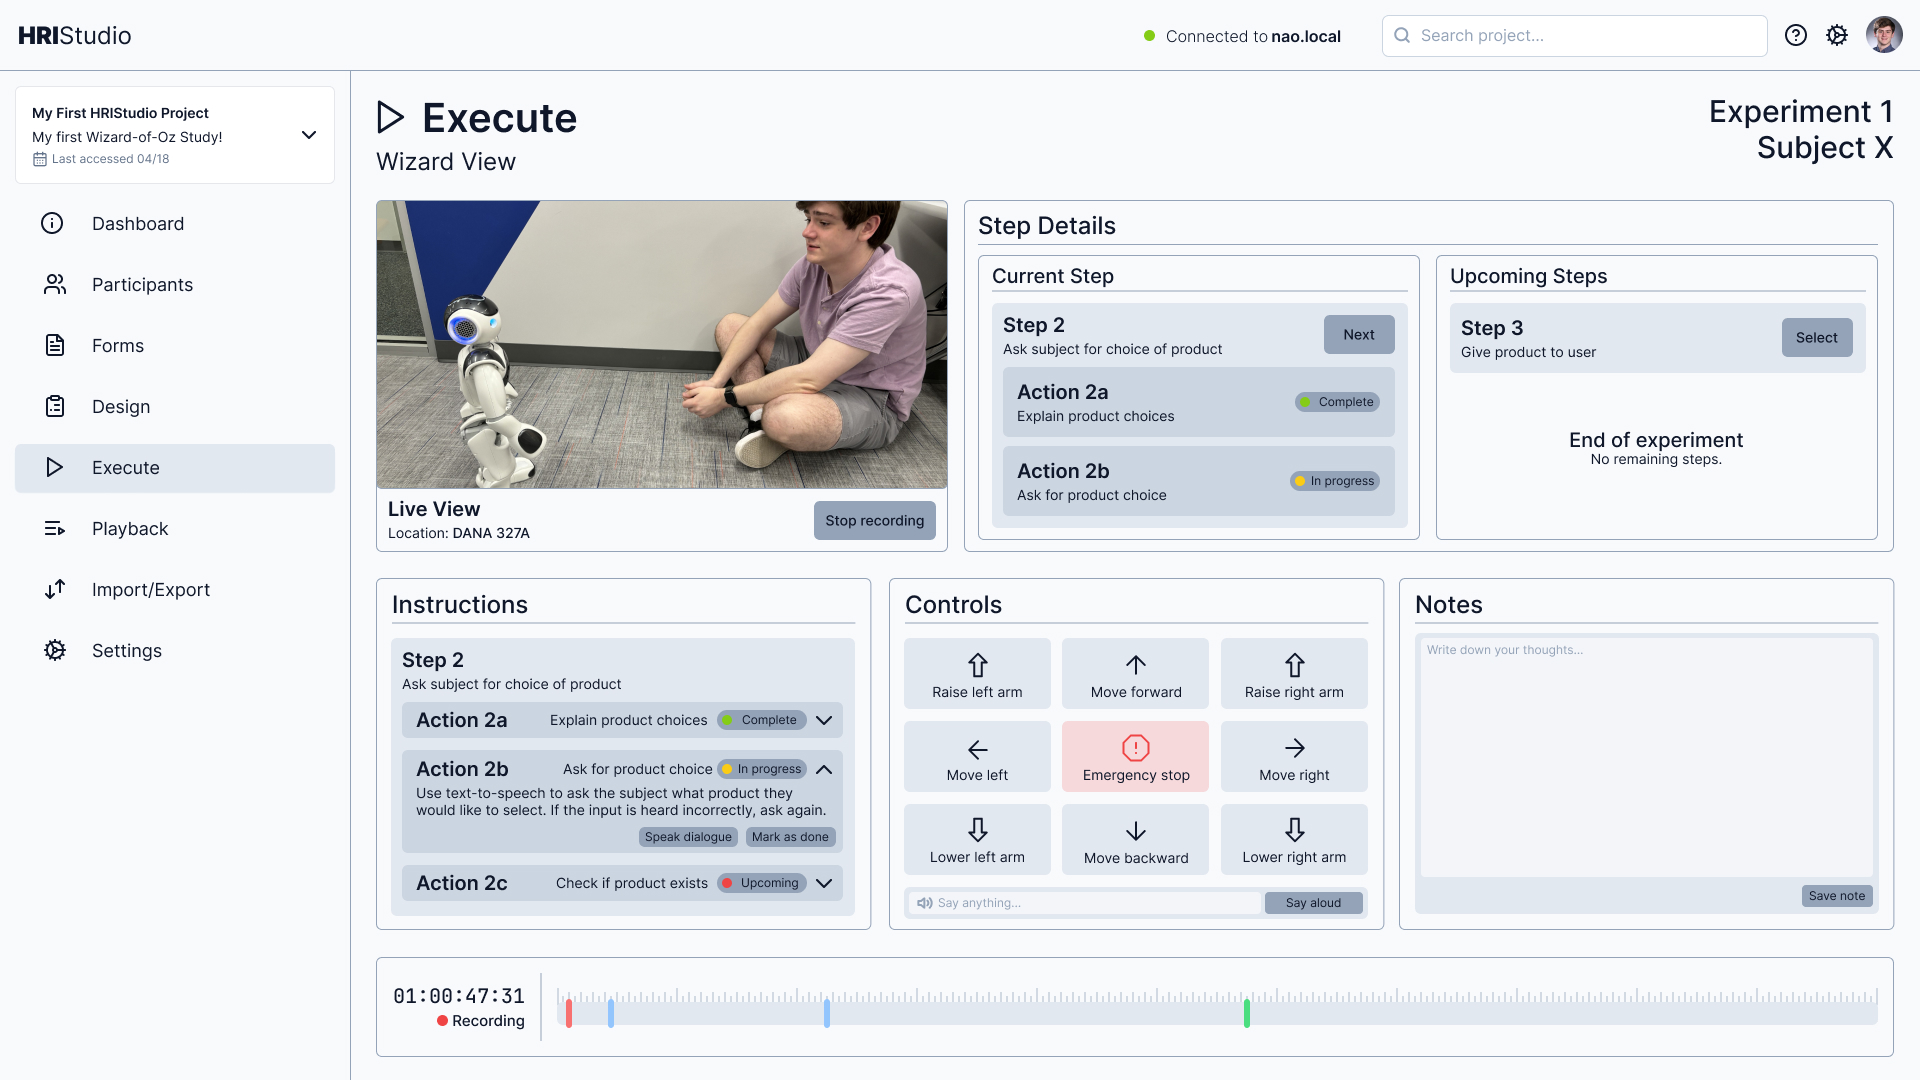
\includegraphics[width=0.4\paperwidth]{assets/mockups/execute}
         \vskip -0.3cm
        \caption{The wizard's \emph{Execute} view during a live experiment}
        \label{fig:execute}
    \end{center}
    \vskip -0.5cm
\end{figure}

As shown in~\ref{fig:playback}, our \emph{Playback} mockups showcase features for synchronized playback of recorded data streams, including audio, video, and applicable sensor data. These mockups incorporate visual and textual annotations, scrubbing capabilities, and data export options to support comprehensive post-experiment analysis and reproducibility.

\begin{figure}[h]
    \begin{center}
        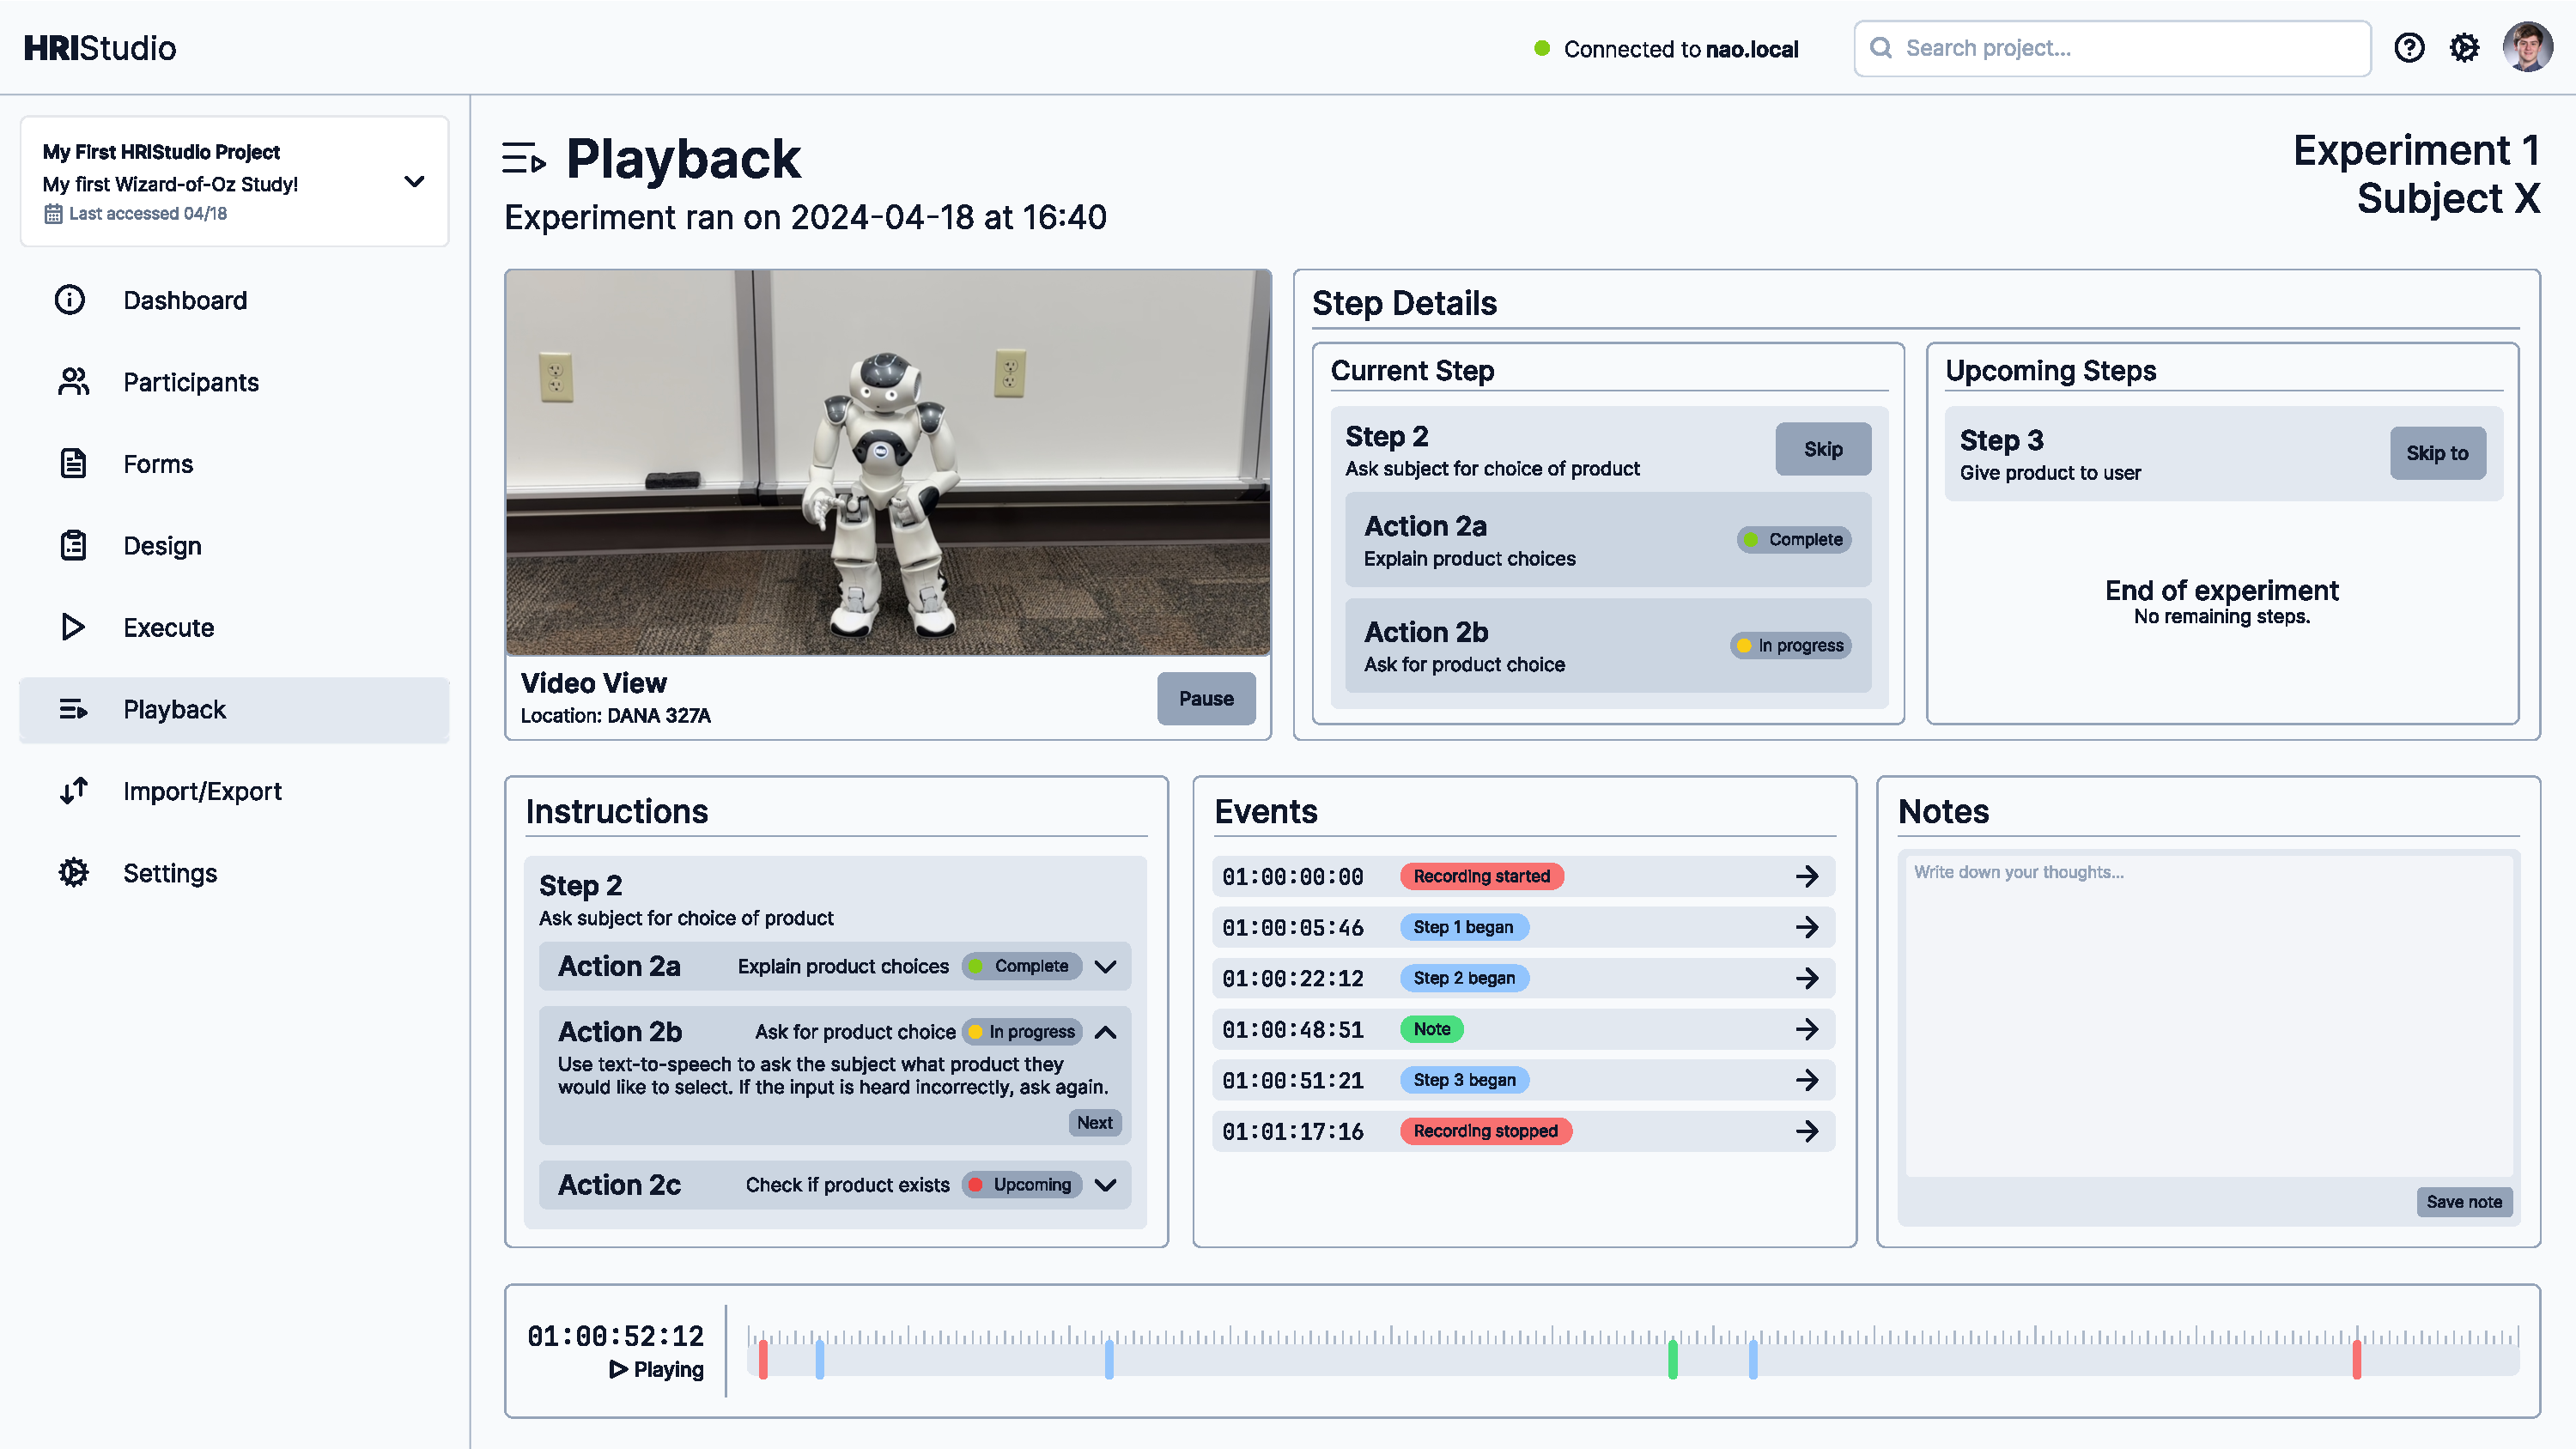
\includegraphics[width=0.4\paperwidth]{assets/mockups/playback}
        \vskip -0.3cm
        \caption{The \emph{Playback} view of an experiment within a study}
        \label{fig:playback}
    \end{center}
    \vskip -0.7cm
\end{figure}

\subsection{Development roadmap}

While the UI mockups have laid a solid foundation, we anticipate challenges in transforming these designs into a fully functional platform, such as integrating the Next.js web application with the ROS interface and handling bi-directional communication between the two. We plan to leverage tRPC for real-time data exchange and robot control.

Another key challenge is developing the \emph{Design} view's visual programming environment, and encoding procedures into a shareable format. We will explore existing visual programming libraries and develop custom components for intuitive experiment construction.

Implementing robust data logging and synchronized playback of audio, video, and sensor data while ensuring efficient storage and retrieval is also crucial.

To address these challenges, our development roadmap includes:
\begin{itemize}
    \item Establishing a stable Next.js codebase with tRPC integration,
    \item Implementing a ROS interface node for robot communication,
    \item Developing the visual experiment designer,
    \item Integrating data logging for capturing experimental data streams,
    \item Building playback and annotation tools with export capabilities,
    \item Creating tutorials and documentation for researcher adoption.
\end{itemize}

This roadmap identifies some of the challenges ahead. We expect that this plan will fully realize HRIStudio into a functional and accessible tool for conducting WoZ experiments. We hope for this tool to become a significant aid in HRI research, empowering researchers and fostering collaboration within the community. 

\bibliography{refs}
\bibliographystyle{plain}

\end{document}
